\part{Embedded Walls}

trois types de sytructure retenant le sol:
\begin{center}
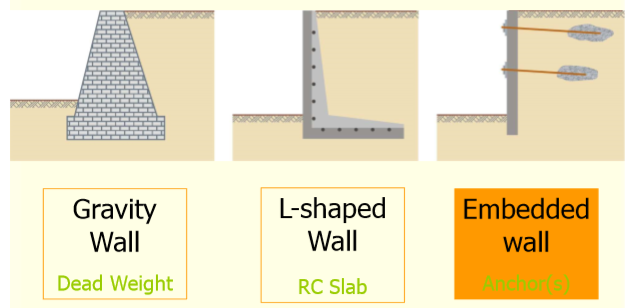
\includegraphics [scale=0.5]{pictures/1.PNG}
\end{center}

\section{Pression des terres et de l'eau}

Voir cours de géotechnique 2.

Voici un rapide résumé, le sol peut être en trois états possible, actif ($K_a$), passif($K_p$) et neutre ($K_0$). Ces coefficient permetent de passer d'une force verticale à une force horizontale :

$$ K = \frac{\delta'h}{\delta'z}$$

Pour la pression de l'eau, voir le cours de géotechnique 1. Ce qui nous intéresse ici, c'est la pression de l'eau sur un mur à sa base (Renard).

\begin{center}
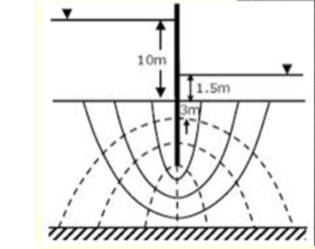
\includegraphics [scale=0.5]{pictures/2.PNG}
\end{center}

\section{Type d'écrans}

\subsection{Blindages des fouilles et excavation}

différentes solutions:
\begin{itemize}
    \item le blindage par planches verticales: possible uniquement dans le cas de sol non pulvérulent. Il suffit de creuser un mètre (=une passe), mettre des parois verticales, les étançonner et recommencer.
    \item le blindage par planches horizontales: pareil mais les planches sont horizontales
    \item la paroi berlinoise: utile pour excaver de grandes hauteurs et que la fouille est large. On enfonce des poutrelles en acier jusqu'à 1 mètre sous la profondeur de la fouille, on descend en y insérant des planches.
\end{itemize}

\medskip

\subsection{Palplanches}

On insère dans le sol avant l'excavation des palplanches. Elles sont battues, lancées ou vibrées dans le sol. On place des étançons ou des tirants au fur et à mesure de la fouille. Il en existe deux sortes, les plates (effort de traction horizontaux) et les modules (reprend de la flexion) (agrafées à la fibre neutre (U) (symétrique donc moins de déviation) ou à la fibre extrême (z) (pas de risque de glissement car $\theta = 0$). Une cellule de palplanche fermée est appelé gabion.

Essentiellement utilisé pour des terrains aquifère et pour des construction hydraulique. Peut utilisé en ville (vibration, bruit, ...).

\subsection{Parois moulées}

Réalisé par panneau séparé, un panneau puis l'autre et on creuse au milieu.
Méthode:
\begin{itemize}
    \item Réalise un muret guide
    \item Creuse avec un grappin ou une hydro-fraise (ce nom est trop stylé). Durant l'excavation, on injecte de la boue thixotropique pour éviter l'éboulement
    \item On place des tubes-joint pour délimiter la largeur des panneaux.
    \item On place les armatures
    \item On coule le béton (plus lourd que la boue qui remonte)
    \item On retire les tubes-joint avec des vérins hydrauliques.
\end{itemize}

\medskip

\underline{boue thixotropique:} boue qui se solidifie au repos et se liquéfie lorsqu'elle est agitée. Elle tapisse les parois de l'excavation et pénètre dans le sol pour former un cake imperméable, ce qui stabilise le sol. Elle entre par pression hydrostatique dans le sol ($\gamma = 11 kN/m^3$).

\subsection{Alignement de pieux}

Mis en place avant excavation. trois dispositifs: 
\begin{itemize}
    \item Pieux sécants: on force un troisième pieux entre deux précédemment installé par forage.
    \item Pieux tangents: les pieux se touchent juste.
    \item Pieux clairsemés: pas de contact.
\end{itemize}

\section{Stabilité des écrans}

Les murs de soutènement peuvent adopter trois types de comportement:
\begin{itemize}
    \item A: Cas isostatique d'un mur sans ancre à sa tête et restreint ("clamped") à sa base.
    \item B: Cas isostatique d'un mur avec une ancre à sa tête et simplement posé à sa base.
    \item C: Cas Hyperstatique d'un mur avec une ancre à sa tête et restreint à sa base.
\end{itemize} 

\medskip

Pour dimensionner ces différents cas, on utilise la méthode de Rankine pour un sol pulvérulent. On utilisera deux équations: l'équilibre de rotation autour du pied et l'équilibre horizontal.

\subsection{Cas A: Isostatic case of wall without anchor at head and clamped at toe}

\begin{center}
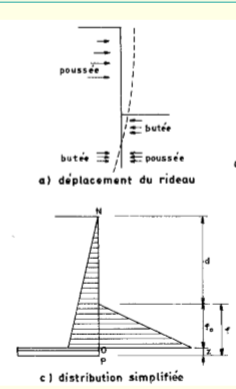
\includegraphics [scale=0.8]{pictures/12.PNG}
\end{center}

On considère que le rideau pivote autour d'un axe situé légèrement au-dessus de son extrémité inférieur. On accorde peu d'importance à la partie décomprimé en dessous du pivot car négligeable. Pour les besoins de calcul, on remplace la distribution des contraintes par une distribution plus simple.

On a deux inconnues: 
\begin{itemize}
    \item La profondeur ou la pression est inversée (f)
    \item la counter passive reaction (CB)
\end{itemize}

\medskip

\begin{center}
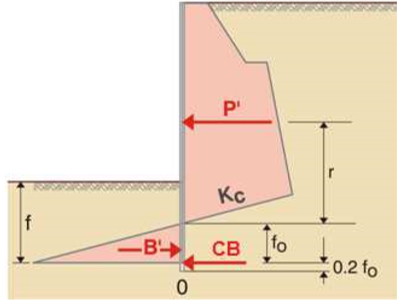
\includegraphics [scale=0.8]{pictures/36.PNG}
\end{center}

Pour résoudre ce problème, on suppose dans un premier temps que la résultante de la contre butée CB s'applique au point 0. Dans un second temps, on allongera la fiche ainsi obtenu pour donner à la contre butée une longueur matérielle sur laquelle elle pourra s'appliquer ($0.2f_0$).

Grâce à l'équilibre de rotation autour du point de contre butée:

\begin{center}
\begin{tabular}{c|c}
    $(f_0 + r)P' = \frac{f_0}{3}\frac{\gamma f_0}{2} K_c$    
                        &  P': résultante des forces à droite \\
    $Kc = K_p - K_a$    &  B': résultante des forces à gauches \\
                        &  $K_c$: pente du diagramme résultant des pressions nettes
\end{tabular}
\end{center}

\medskip
On peut alors calculer $f_0$ en tenant compte de la charge triangulaire de la partie inférieure:
$$ B'=\frac{K_c \gamma f_0^2}{2}$$

Plusieur corrections sont à apporter au diagramme, dans le cadre du cours on acceptera d'adopter la méthode compensatoire consistant à allonger de 20\% la fiche (0.2 $f_0$).

\subsection{Cas B: Isostatic case of wall with anchor at head and simply supported at toe}

Deux inconnues: la fiche $f_0$ et l'effort d'ancrage T. La somme des moments étant nulle au point d'ancrage (on élimine T), on obtient une équation du troisième degré en f, on obtient donc $f_0$. Le calcul de T est alors immédiat.

Le moment maximal se produit le plus souvent vers le bas de la partie libre de la palplanche ou vers le milieu de la longueur compté entre l'ancrage et le centre des réactions d'appuis.

La butée du terrain est la seule force qui empêche la palplanche de pivoter. Il est donc indispensable d'introduire un coefficient de sécurité (2) ou de multiplier la longueur de la fiche par $\sqrt{2}$ (on augmente bien la valeur de la butée mais aussi légèrement la poussée).

\begin{center}
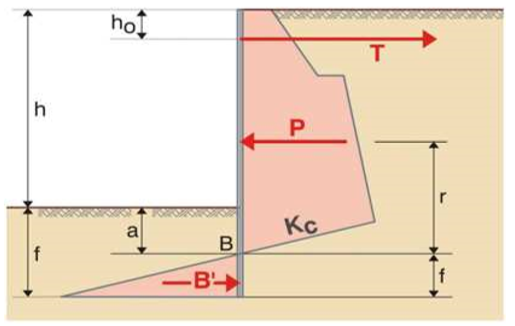
\includegraphics [scale=0.8]{pictures/38.PNG}
\end{center}

$$(h+a-h_0-r)P =(h+a-h_0+\frac{2}{3}f_0)\frac{\gamma f^2}{2}K_c$$ 

$$ B'=\frac{K_c \gamma f^2}{2} $$
$$ T = P - B'$$

\subsection{Cas C: Hyperstatic case of wall with anchor at head and clamping at toe}

\subsubsection{Méthode de la ligne élastique}

On a trois inconnues: profondeur ($f_0)$, ancrage (T) et contrebutée (CB). 
Pour le résoudre, on fait une hypothèse: le pied de la palplanche reste immobile et la tangente à la palplanche en ce point reste verticale au point d'ancrage. cette méthode est très longue.

\subsubsection{Méthode de Blum (poutres équivalentes)}

On pose une rotule au point R situé légèrement en dessous du fond de fouille. La ou le moment fléchissant est nul. M = 0 à la rotule ($\Delta \sigma_h = 0$). On considère donc deux murs isostatique [SU] et [UO].

La partie [SU] peut être calculé comme une poutre isolée reposant sur deux appuis: au point de moment nul et au point d'ancrage.

La partie [UO] peut être calculé comme une poutre isolée de portée inconnue reposant sur deux appuis: au point de moment nul et au point d'action de contrebutée (on connait Rt).

Finalement on adoptera $f=1.2f_0$

\begin{center}
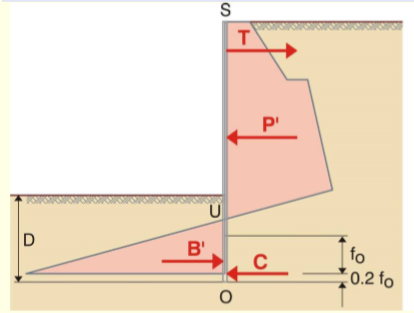
\includegraphics [scale=0.8]{pictures/43.PNG}
\end{center}

On peut apparemment calculer que $B'=3R=\frac{K_c \gamma f_0^2}{2}$ sans doute par une égalité de force ou de moment.

\subsection{Gabions}

Ce sont des cellules en grillage (ou sheet pile) qui contiennent des cailloux. Elles agissent comme des structures poids.

$$ \delta'_h = A \gamma' h $$   et    $$ N=A \gamma'h\frac{D}{2}$$ 

On étudie la stabilité en deux points: 
\begin{itemize}
    \item T: condition de stabilité est $\frac{h}{D} \leq \frac{\pi tan(\phi)}{2A}$ (glissement)
    \item R: condition de stabilité est $\frac{h}{D} \leq \sqrt{\frac{3 \pi}{16 A}}$ (renversement)
\end{itemize}

\begin{center}
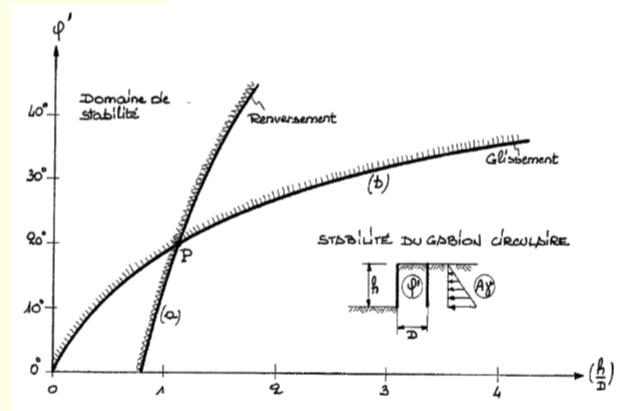
\includegraphics [scale=0.8]{pictures/158.PNG}
\end{center}
